\documentclass[a4paper, 12pt]{article}

\usepackage{graphicx}
\usepackage{longtable}
\graphicspath{ {images/} }

\newcommand{\templates}{../../template}
\usepackage[a4paper, margin=2.5cm]{geometry}

\usepackage{enumitem}
\setlist[itemize]{noitemsep}
\setlist[enumerate]{noitemsep}

\let\oldpar\paragraph
\renewcommand{\paragraph}[1]{\oldpar{#1\\}\noindent}
\usepackage{graphicx}
\usepackage{hyperref}
\usepackage{makecell}

\newcommand{\settitolo}[1]{\newcommand{\titolo}{#1\\}}
\newcommand{\setprogetto}[1]{\newcommand{\progetto}{#1\\}}
\newcommand{\setcommittenti}[1]{\newcommand{\committenti}{#1\\}}
\newcommand{\setredattori}[1]{\newcommand{\redattori}{#1\\}}
\newcommand{\setrevisori}[1]{\newcommand{\revisori}{#1\\}}
\newcommand{\setresponsabili}[1]{\newcommand{\responsabili}{#1\\}}
\newcommand{\setversione}[1]{
	\ifdefined\versione\renewcommand{\versione}{#1\\}
	\else\newcommand{\versione}{#1\\}\fi
}
\newcommand{\setdestuso}[1]{\newcommand{\uso}{#1\\}}
\newcommand{\setdescrizione}[1]{\newcommand{\descrizione}{#1\\}}

\newcommand{\makefrontpage}{
	\begin{titlepage}
		\begin{center}

		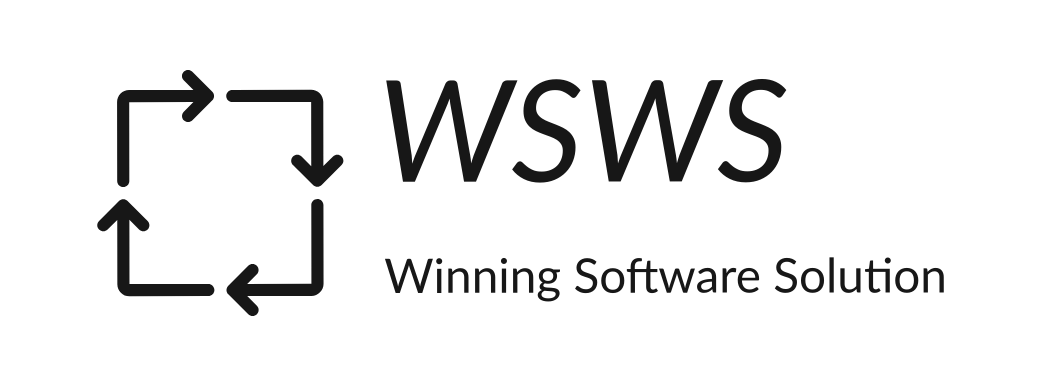
\includegraphics[width=0.4\textwidth]{../../template/WSWS-logos_transparent_crop}\\

		{\Large Winning Software Solution}\\[6pt]
		\href{mailto://winningsoftwaresolution@gmail.com}{winningsoftwaresolution@gmail.com}\\
		
		\ifdefined\progetto
		\vspace{1cm}
		{\Large\progetto}
		{\large\committenti}
		\else\fi
		
		\vspace{1.5cm}
		{\LARGE\titolo}
		
		\vfill
		
		\begin{tabular}{r | l}
		\multicolumn{2}{c}{\textit{Informazioni}}\\
		\hline
		
		\ifdefined\redattori
			\textit{Redattori} &
			\makecell[l]{\redattori}\\
		\else\fi
		\ifdefined\revisori
			\textit{Revisori} &
			\makecell[l]{\revisori}\\
		\else\fi
		\ifdefined\responsabili
			\textit{Respondabili} &
			\makecell[l]{\responsabili}\\
		\else\fi
		
		\ifdefined\versione
			\textit{Versione} & \versione
		\else\fi
		
		\textit{Uso} & \uso
		
		\end{tabular}
		
		\vspace{2cm}
		
		\ifdefined\descrizione
		Descrizione
		\vspace{6pt}
		\hrule
		\descrizione
		\else\fi
		\end{center}
	\end{titlepage}
}
\usepackage{hyperref}
\usepackage{array}
\usepackage{tabularx}

\def\vers#1-#2-#3-#4-#5\\{#1&#2&#3&#4&#5\\\hline}

\newcommand{\addversione}[5]{
	\ifdefined\versioni
		\let\old\versioni
		\renewcommand{\versioni}{#1&#2&#3&#4&#5\\\hline\old}
	\else
		\newcommand{\versioni}{#1&#2&#3&#4&#5\\\hline}
	\fi
}

\newcommand{\setversioni}[1]{\newcommand{\versioni}{#1}}

\newcommand{\makeversioni}{
	\begin{center}
		\begin{tabularx}{\textwidth}{|c|c|c|c|X|}
		\hline
		\textbf{Versione} & \textbf{Data} & \textbf{Persona} & \textbf{Attivtà} & \textbf{Descrizione} \\
		\hline
		\versioni
		\end{tabularx}
	\end{center}
	\clearpage
}

\settitolo{Analisi dei requisiti}
\setprogetto{ShopChain}
\setcommittenti{SyncLab}
\setredattori{Alberto Nicoletti, Andrea Volpe}
\setdestuso{esterno}
\setdescrizione{
Analisi dei requisiti del progetto ShopChain con casi d'uso e requisiti.
}

\addversione{0.0.0}{11/12/2021}{Alberto Nicoletti}{Redazione}{Struttura del documento, stesura sezioni 1 e 2}
\addversione{0.0.1}{30/12/2021}{Alberto Nicoletti}{Redazione}{Stesura casi d'uso da UC1 a UC5.4}
\addversione{0.0.2}{03/01/2022}{Andrea Volpe}{Redazione}{Stesura casi d'uso da UC6 a UC20}
\addversione{0.0.3}{03/01/2022}{Alberto Nicoletti}{Redazione}{Aggiunta immagini}
\addversione{0.0.4}{12/01/2022}{Andrea Volpe}{Redazione}{Rimozione/aggiunta casi d'uso}
\addversione{0.0.5}{16/01/2022}{Alberto Nicoletti}{Redazione}{Stesura primi requisiti}

\begin{document}

\makefrontpage

\makeversioni

\section{Introduzone}
\subsection{Scopo del documento}
Lo scopo del documento è raccogliere i risultati dell'attività di analisi dei requisiti. Contiene quindi la descrizione dei casi d'uso del prodotto software da sviluppare, ed i requisiti suddivisi per tipologia. Si vuole così dimostrare una completa comprensione del problema e delle aspettative  nella soluzione. I casi d'uso, ma soprattuto i requisiti saranno tenunuti in considerazione nelle fasi di progettazione e di verifica. 
\subsection{Glossario}
Di seguito un elenco di parole usate in questo documento, la cui definizione può essere trovata nel Glossario.
parola, parola, parola.

\section{Descrizione del prodotto}
L'azieda \textit{SyncLab} propone, attraverso il capitolato C2: \textit{ShopChain - Exchange Platform on
BlockChain}. Consiste nel realizzare un prototipo di una piattaforma in grado di ‘affiancare’ un crypto-e-commerce nella fasi di pagamento fino alla consegna.
\subsection{Scopo del prodotto}
Il progetto consiste nello sviluppo di una piattaforma su blockchain con lo scopo di rendere possibile e in sicurezza l'acquisto di prodotti tramite criptovalute. Il processo di trasferimento del denaro avviene seguendo queste fasi:
\begin{enumerate}
\item Caricamento dei dati dell'ordine di acquisto nella blockchain e generazione dello smart contract.
\item Trasferimento del denaro dal wallet dell'acquirente in blockchain.
\item Notifica al venditore dell'avvenuto pagamento e blocco del denaro in blockchain.
\item Conferma di ricezione del pacco da parte dell'acquirente tramite scannerizzazione di un Qr Code nel prodotto acquistato.
\item Sblocco del denaro e trasferimento nel wallet del venditore.
\end{enumerate}
\subsection{Parti del prodotto}
Il prodotto software è composta dalle seguenti parti:
\begin{itemize}
\item Smart contracts nella blockchain per la gestione di tutte le fasi del processo di trasferimento del denaro.
\item Piattaforma web per la gestione dei pagamenti da parte del venditore.
\item Piattaforma web per la gestione dei pagamenti da parte dell' acquirente.
\item App o web app per la scannerizzazione del Qr code.
\end{itemize}
\subsection{Caratteristiche utenti}
Gli utenti di \textit{ShopChain} possono essere suddivisi in due categorie:
\begin{itemize}
\item Venditore: gli amministratori di un sito di e-commerce che vogliono aggiungere le criptovalute come metodo di pagamento.
\item Acquirente: I clienti di un sito di e-commerce che scelgono di utilizzare le criptovalute come pagamento per i prodotti da acquistare.
\end{itemize}
Tutti gli utenti sono in possesso di un wallet per criptovalute. 
Non potendo prevedere con accuratezza quanti e quali e-commerce decideranno di utilizzare \textit{ShopChain} altre considerazioni sulle caratteristiche di utenza sono irrilevanti. Il prodotto deve essere facilmente integrabile in più tipologie di e-commerce possibili.

\subsection{Vincoli e preferenze}
La proponente non impone vincoli nella scelta della tipologia di tecnologie, va ci sono comunque delle scelte preferenziali da considerare:
\begin{itemize}
\item Utilizzo di blockchain pubblica
\item utilizzo di Java e Angular per lo sviluppo delle parti di Back-end e di Front-end della componente web application del sistema
\item utilizzo di database Postgres
\end{itemize}

Per il completamento del progetto la proponente richiede che siano realizzati i seguenti risultati:
\begin{itemize}
\item server, completo di UI
\item test che dimostrino il corretto funzionamento dei servizi e delle funzionalità previste, con una copertura minima dell' 80\% correlata di report.
\item documentazione su: scelte implementative e progettuali effettuate e relative motivazioni, problemi aperti e eventuali soluzioni proposte da esplorare.
\end{itemize}

\section{Casi d'uso}

\paragraph{UC1 - Consultazione manuale ShopChain}
\textbf{Attore primario}: Venditore\\
\textbf{Precondizioni}: Il venditore usa il servizio ShopChain e vorrebbe avere più informazioni sul suo utilizzo.\\
\textbf{Postcondizioni}: Il venditore consulta il manuale utente di ShopChain.\\
\textbf{Scenario principale}:\\
\begin{enumerate}
\item Al venditore viene fornito il manuale utente già dall'acquisizione del prodotto ShopChain.
\item Il venditore è libero di consultare il manuale in ogni momento.
\end{enumerate}

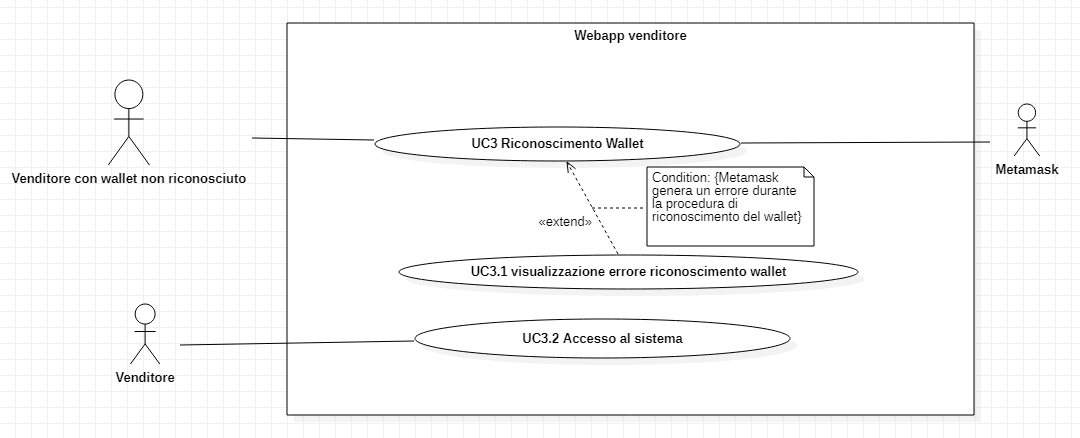
\includegraphics[width=0.9\textwidth]{UseCase_venditore2.png}

\paragraph{UC2 - Riconoscimento wallet}
\textbf{Attore primario}: Venditore privo di wallet riconosciuto.\\
\textbf{Attore secondario}: Metamask.\\
\textbf{Precondizioni}: Il venditore ha aperto la webapp e non si è ancora fatto riconoscere il wallet da Metamask.\\
\textbf{Postcondizioni}: Il venditore ha fatto riconoscere il wallet a Metamask e accede al sistema.\\
\textbf{Scenario principale}:
\begin{enumerate}
    \item Il venditore apre la webapp.
    \item Il venditore fa riconoscere tramite Metamask il proprio wallet.
    \item Il venditore ha un wallet associato e accede al sistema.
\end{enumerate}
\textbf{Estensioni}:
\begin{enumerate}
    \item UC2.1 Metamask genera un errore durante la procedura di riconoscimento del wallet.
    \begin{enumerate}
        \item Il sistema mostra l'errore riconoscimento wallet non riuscito.
        \item Il sistema mostra il messaggio riprovare.
        \item Il sistema ripete UC2.
    \end{enumerate}
\end{enumerate}

\paragraph{UC2.2 - Accesso al sistema}
\textbf{Attore primario}: Venditore con wallet associato.\\
\textbf{Precondizioni}: Il venditore apre la webapp e si è già fatto riconoscere il wallet da Metamask.\\
\textbf{Postcondizioni}: Il venditore accede al sistema.\\
\textbf{Scenario principale}:
\begin{enumerate}
    \item Il venditore fa riconoscere tramite Metamask il proprio wallet.
    \item Il venditore apre la webapp.
    \item Il venditore ha un wallet associato e accede al sistema.
\end{enumerate}

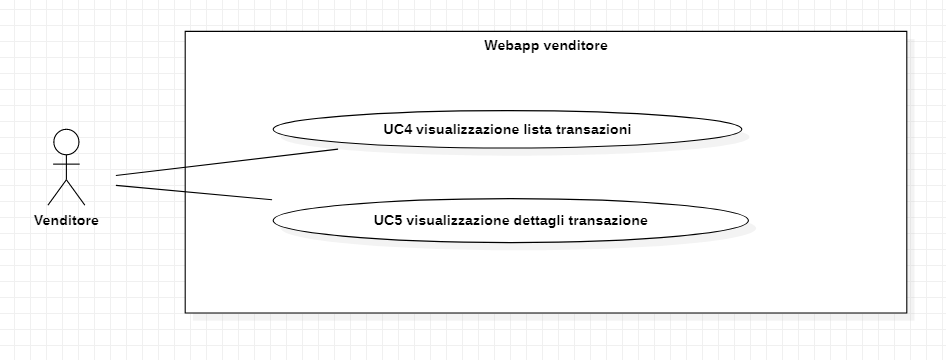
\includegraphics[width=0.9\textwidth]{UseCase_venditore3.png}

\paragraph{UC3 visualizzazione lista transazioni}
\textbf{Attore primario}: Venditore \\
\textbf{Precondizioni}: Il venditore ha effettuato l'accesso al sistema.\\
\textbf{Postcondizioni}:  Il venditore vede la lista delle transazioni
Scenario principale.\\
\textbf{Scenario principale}:
\begin{enumerate}
\item Il venditore tramite un menu arriva alla lista delle transazioni.
\item Il venditore può scegliere che tipo di transazioni vedere (tutte, completate, in attesa).
\item Il sistema mostra al venditore l'elenco delle transizioni richieste, ordinate per data e per ognuna vengono mostrati i dati più importanti.
\end{enumerate}

\paragraph{UC4 - visualizzazione dettaglio transazione}
\textbf{Attore primario}: Venditore\\
\textbf{Precondizioni}: Il venditore ha acceduto alla funzionalità di visualizzazione della lista delle transazioni.\\
\textbf{Postcondizioni}: Il venditore vede i dettagli di una singola transizione.\\
\begin{enumerate}
\item Il venditore seleziona una delle transizioni dall'elenco.
\item Il venditore visualizza i dettagli della singola transizione.
\end{enumerate}

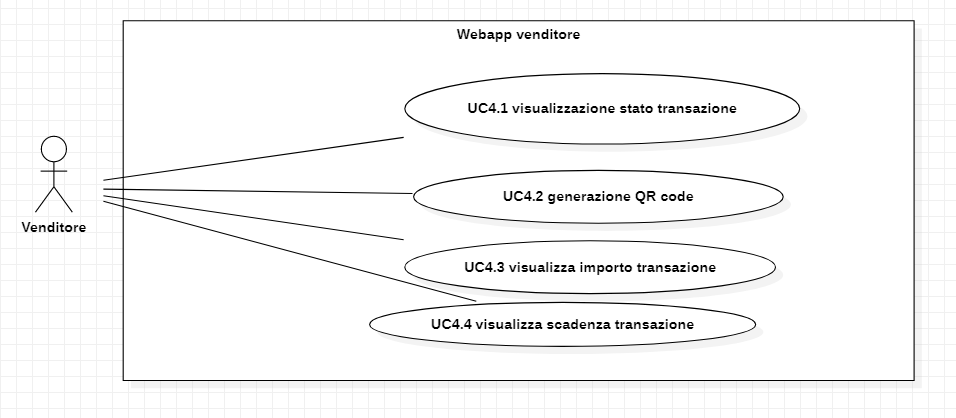
\includegraphics[width=0.9\textwidth]{UseCase_venditore4.png}

\paragraph{4.1 - Visualizzazione stato transizione}
\textbf{Attore primario}: Venditore\\
\textbf{Precondizioni}: Il venditore vuole visualizzare lo stato di una transizione.\\
\textbf{Postcondizioni}: Il venditore visualizza lo stato di una transizione.\\
\textbf{Scenario principale}: Il venditore vede se la transizione è in attesa, oppure è stata completata.\\

\paragraph{UC4.2 - Generazione QR Code}
\textbf{Attore primario}: Venditore\\
\textbf{Precondizioni}: Il venditore vuole generare il QR Code di una transizione in attesa.\\
\textbf{Postcondizioni}: Il venditore è in possesso del QR code da applicare sul pacco del prodotto.\\
\begin{enumerate}
\item Il venditore visualizza il Qr code della transizione in attesa selezionata.
\item Il venditore stampa il Qr code e lo appplica sul pacco del prodotto.
\end{enumerate}

\paragraph{UC4.3 - Visualizzazione importo transazione}
\textbf{Attore primario}: Venditore\\
\textbf{Precondizioni}: Il venditore vuole visualizzare l'importo di una transizione.\\
\textbf{Postcondizioni}: Il venditore visualizza l'importo di una transizione.\\
\textbf{Scenario principale}: Il venditore vede l'importo della transazione.\\

\paragraph{UC4.4 - Visualizzazione scadenza transazione}
\textbf{Attore primario}: Venditore\\
\textbf{Precondizioni}: Il venditore vuole visualizzare la scadenza di una transazione in attesa.\\
\textbf{Postcondizioni}: Il venditore visualizza la scadenza di una transazione in attesa.\\
\textbf{Scenario principale}: Il venditore vede la data della scadenza di una transazione in attesa, oltre la quale riceverà l'importo anche se non è stato scannerizzato il QR Code.\\

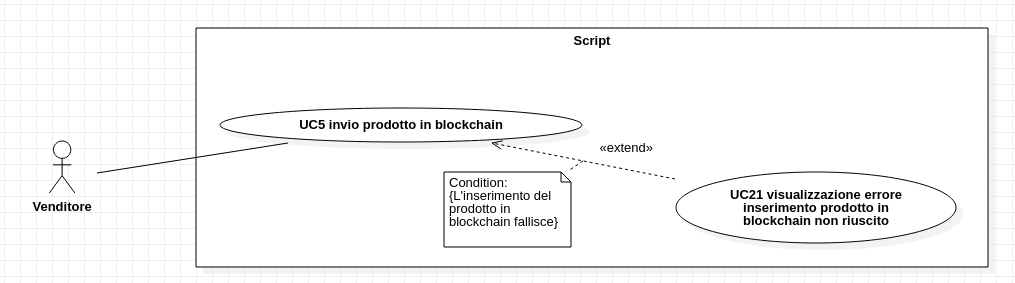
\includegraphics[width=0.9\textwidth]{UseCase_script1}

\paragraph{UC5 - Inserimento prodotto in blockchain}
\textbf{Attore primario}: Venditore.\\
\textbf{Precondizioni}: Il venditore ha integrato lo script nell'e-commerce e ha inserito un nuovo prodotto nell'e-commerce.\\
\textbf{Postcondizioni}: Il venditore ha inserito il nuovo prodotto in blockchain.\\
\textbf{Scenario principale}:
\begin{enumerate}
    \item Il venditore integra nel backend del proprio e-commerce lo script fornito da noi.
    \item Il venditore inserisce un nuovo prodotto nell'e-commerce.
    \item Tramite lo script il prodotto viene inviato in blockchain.
    \item Il prodotto è inserito in blockchain.
\end{enumerate}
\textbf{Estensioni}:
\begin{enumerate}
    \item UC21 L'invio del prodotto in blockchain fallisce.
    \begin{enumerate}
        \item Lo script salva in un file di log il messaggio di errore.
    \end{enumerate}
\end{enumerate}

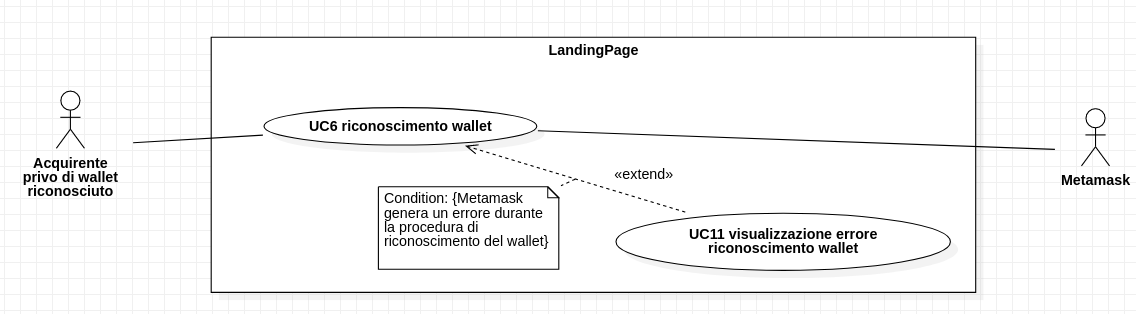
\includegraphics[width=0.9\textwidth]{UseCase_landing_page1}

\paragraph{UC6 - Riconoscimento wallet}
\textbf{Attore primario}: Acquirente privo di wallet riconosciuto.\\
\textbf{Attore secondario}: Metamask.\\
\textbf{Precondizioni}: L'acquirente ha aperto la landing page e non si è ancora fatto riconoscere il wallet da Metamask.\\
\textbf{Postcondizioni}: L'acquirente ha fatto riconoscere il wallet a Metamask e accede al sistema.\\
\textbf{Scenario principale}:
\begin{enumerate}
    \item L’utente apre la landing page.
    \item L’utente fa riconoscere tramite Metamask il proprio wallet.
    \item L’utente ha un wallet associato e accede al sistema.
\end{enumerate}
\textbf{Estensioni}:
\begin{enumerate}
    \item UC11 Metamask genera un errore durante la procedura di riconoscimento del wallet.
    \begin{enumerate}
        \item Il sistema mostra l'errore riconoscimento wallet non riuscito.
        \item Il sistema mostra il messaggio riprovare.
        \item Il sistema ripete UC6.
    \end{enumerate}
\end{enumerate}

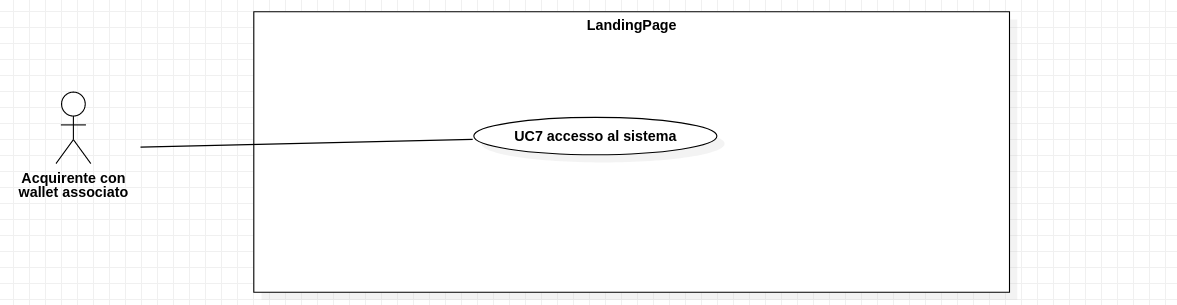
\includegraphics[width=0.9\textwidth]{UseCase_landing_page2}

\paragraph{UC7 - Accesso al sistema}
\textbf{Attore primario}: Acquirente con wallet associato.\\
\textbf{Precondizioni}: L'acquirente apre la landing page e si è già fatto riconoscere il wallet da Metamask.\\
\textbf{Postcondizioni}: L'acquirente accede al sistema.\\
\textbf{Scenario principale}:
\begin{enumerate}
    \item L'acquirente fa riconoscere tramite Metamask il proprio wallet.
    \item L'acquirente apre la landing page.
    \item L'acquirente ha un wallet associato e accede al sistema.
\end{enumerate}

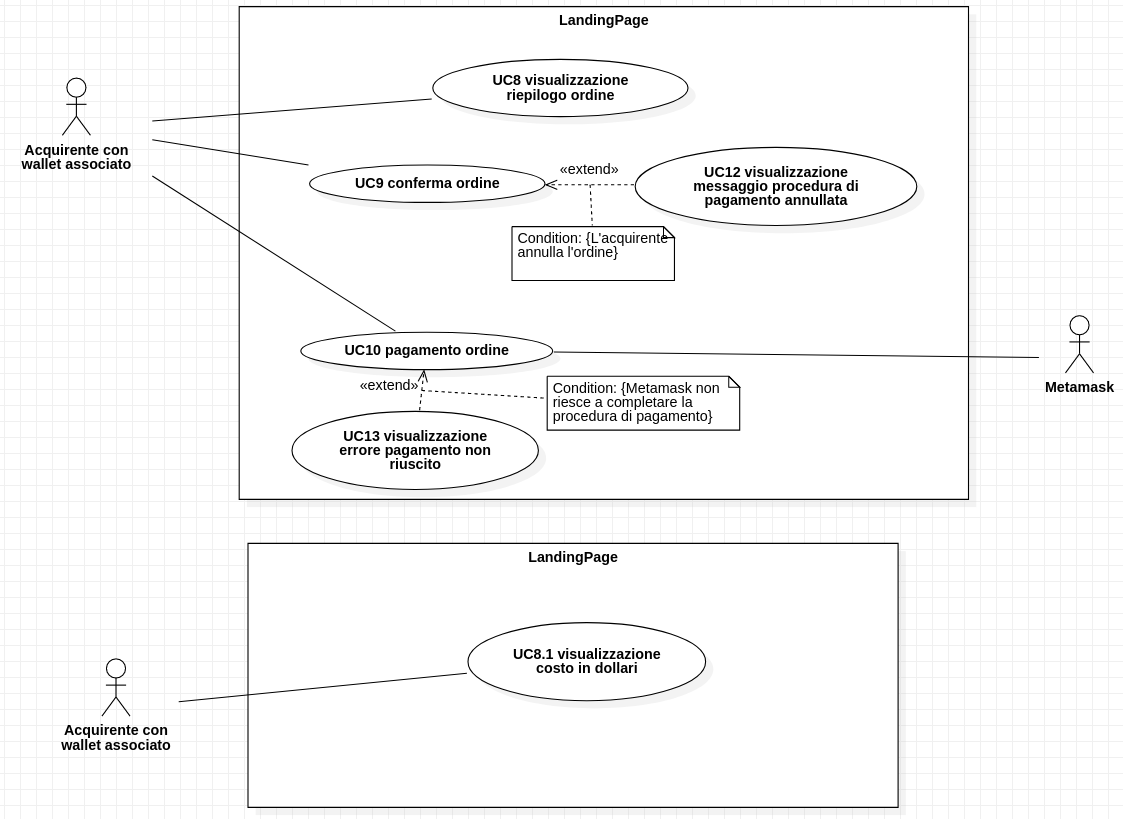
\includegraphics[width=0.9\textwidth]{UseCase_landing_page3}

\paragraph{UC8 - Visualizzazione riepilogo ordine}
\textbf{Attore primario}: Acquirente con wallet associato.\\
\textbf{Precondizioni}: L'acquirente è acceduto al sistema e ha un wallet associato.\\
\textbf{Postcondizioni}: Il sistema mostra il riepilogo dell'ordine.\\
\textbf{Scenario principale}:
\begin{enumerate}
    \item L’utente accede al sistema con un wallet associato.
    \item Il sistema mostra il riepilogo dell'ordine.
\end{enumerate}

\paragraph{UC8.1 - Visualizzazione costo in dollari}
\textbf{Attore primario}: Acquirente con wallet associato.\\
\textbf{Precondizioni}: L'acquirente è acceduto al sistema e ha un wallet associato.\\
\textbf{Postcondizioni}: Il sistema mostra il costo in dollari.\\
\textbf{Scenario principale}:
\begin{enumerate}
    \item L’utente accede al sistema con un wallet associato.
    \item Il sistema mostra il costo in dollari.
\end{enumerate}

\paragraph{UC9 - Conferma ordine}
\textbf{Attore primario}: Acquirente con wallet associato.\\
\textbf{Precondizioni}: Il sistema mostra il riepilogo dell'ordine.\\
\textbf{Postcondizioni}: L'acquirente ha confermato l'ordine.\\
\textbf{Scenario principale}:
\begin{enumerate}
    \item Il sistema mostra il riepilogo dell'ordine.
    \item L'acquirente conferma l'ordine.
\end{enumerate}
\textbf{Estensioni}:
\begin{enumerate}
    \item UC12 L'acquirente annulla l'ordine.
    \begin{enumerate}
        \item Visualizzazione messaggio procedura di pagamento annullata.
        \item Cancellazione sessione di pagamento.
    \end{enumerate}
\end{enumerate}

\paragraph{UC10 - Pagamento ordine}
\textbf{Attore primario}: Acquirente con wallet associato.\\
\textbf{Attore secondario}: Metamask.\\
\textbf{Precondizioni}: L'acquirente ha confermato l'ordine.\\
\textbf{Postcondizioni}: L'acquirente ha pagato l'ordine.\\
\textbf{Scenario principale}:
\begin{enumerate}
    \item L'acquirente avvia la procedura di pagamento.
    \item L'acquirente effettua il pagamento tramite Metamask.
    \item L'ordine è stato pagato.
\end{enumerate}
\textbf{Estensioni}:
\begin{enumerate}
    \item UC13 Metamask non è riuscito a completare la procedura di pagamento.
    \begin{enumerate}
        \item Visualizzazione errore pagamento non riuscito.
        \item Cancellazione sessione di pagamento.
    \end{enumerate}
\end{enumerate}

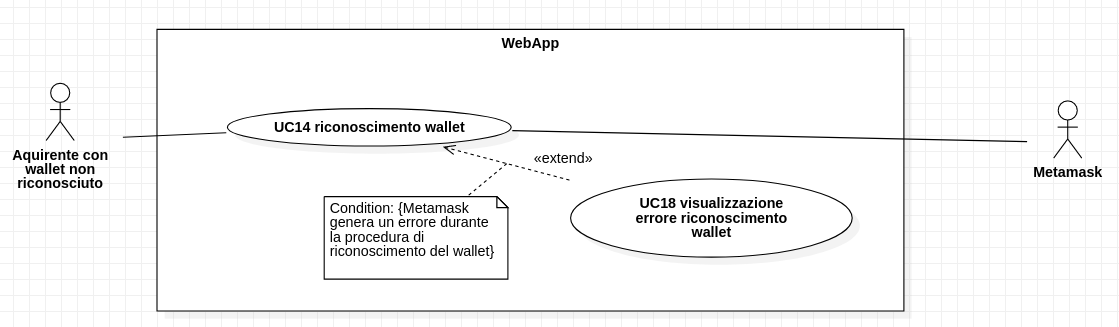
\includegraphics[width=0.9\textwidth]{UseCase_webapp1}

\paragraph{UC14 - Riconoscimento wallet}
\textbf{Attore primario}: Acquirente privo di wallet riconosciuto.\\
\textbf{Attore secondario}: Metamask.\\
\textbf{Precondizioni}: L'acquirente ha aperto la webapp e non si è ancora fatto riconoscere il wallet da Metamask.\\
\textbf{Postcondizioni}: L'acquirente ha fatto riconoscere il wallet a Metamask e accede al sistema.\\
\textbf{Scenario principale}:
\begin{enumerate}
    \item L’acquirente apre la webapp.
    \item L’acquirente fa riconoscere tramite Metamask il proprio wallet.
    \item L’acquirente ha un wallet associato e accede al sistema.
\end{enumerate}
\textbf{Estensioni}:
\begin{enumerate}
    \item UC18 Metamask genera un errore durante la procedura di riconoscimento del wallet.
    \begin{enumerate}
        \item Il sistema mostra l'errore riconoscimento wallet non riuscito.
        \item Il sistema mostra il messaggio riprovare.
        \item Il sistema ripete UC14.
    \end{enumerate}
\end{enumerate}

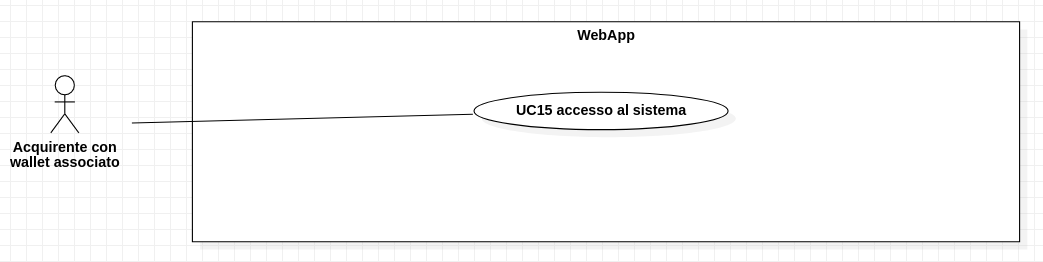
\includegraphics[width=0.9\textwidth]{UseCase_webapp2}

\paragraph{UC15 - Accesso al sistema}
\textbf{Attore primario}: Acquirente con wallet associato.\\
\textbf{Precondizioni}: L'acquirente apre la webapp e si è già fatto riconoscere il wallet da Metamask.\\
\textbf{Postcondizioni}: L'acquirente accede al sistema.\\
\textbf{Scenario principale}:
\begin{enumerate}
    \item L'acquirente fa riconoscere tramite Metamask il proprio wallet.
    \item L'acquirente apre la webapp.
    \item L'acquirente ha un wallet associato e accede al sistema.
\end{enumerate}

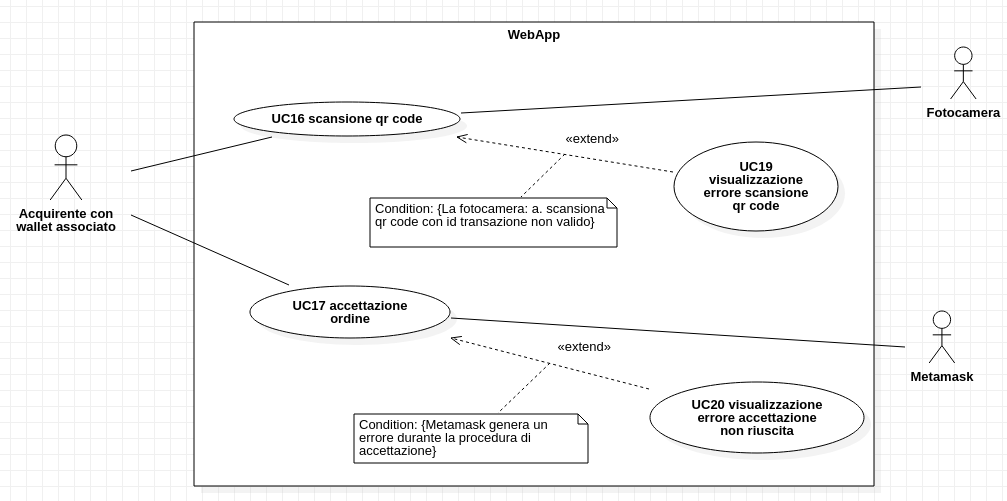
\includegraphics[width=0.9\textwidth]{UseCase_webapp3}

\paragraph{UC16 - Scansione qr code}
\textbf{Attore primario}: Acquirente con wallet associato.\\
\textbf{Attore secondario}: Fotocamera.\\
\textbf{Precondizioni}: L'acquirente ha acceduto al sistema e ha un wallet associato.\\
\textbf{Postcondizioni}: L'acquirente ha scansionato il qr code e il sistema possiede i dati dell'ordine.\\
\textbf{Scenario principale}:
\begin{enumerate}
    \item L'acquirente accede al sistema con un wallet associato.
    \item Il sistema avvia la fotocamera.
    \item L'acquirente scansiona il qr-code.
    \item Il sistema possiede i dati dell'ordine.
\end{enumerate}
\textbf{Estensioni}:
\begin{enumerate}
    \item UC19 La fotocamera ha generato un errore durante la procedura di scansione qr code.
    \begin{enumerate}
        \item La fotocamera ha scansionato un qr code non valido.
        \begin{enumerate}
            \item Il sistema mette in pausa la fotocamera.
            \item Il sistema mostra l'errore nessun qr code non valido.
            \item L'acquirente chiude il messaggio di errore.
            \item Il sistema avvia la fotocamera.
        \end{enumerate}
        \item La fotocamera ha scansionato un qr code valido ma inesistente.
        \begin{enumerate}
            \item Il sistema mette in pausa la fotocamera.
            \item Il sistema mostra l'errore nessun qr code inesistente.
            \item L'acquirente chiude il messaggio di errore.
            \item Il sistema avvia la fotocamera.
        \end{enumerate}
    \end{enumerate}
\end{enumerate}

\paragraph{UC17 - Accettazione ordine}
\textbf{Attore primario}: Acquirente con wallet associato.\\
\textbf{Attore secondario}: Metamask.\\
\textbf{Precondizioni}: L'acquirente ha scansionato un qr code valido.\\
\textbf{Postcondizioni}: L'acquirente ha accettato l'ordine.\\
\textbf{Scenario principale}:
\begin{enumerate}
    \item L'acquirente scansiona un qr code valido.
    \item L'acquirente accetta l'ordine tramite Metamask.
    \item L'acquirente ha accettato l'ordine.
    \item L'acquirente è in possesso dei prodotti dell'ordine.
\end{enumerate}
\textbf{Estensioni}:
\begin{enumerate}
    \item UC20 Metamask genera un errore durante la procedura di accettazione.
    \begin{enumerate}
        \item Il sistema mostra l'errore accettazione non riuscita.
        \item Il sistema mostra il messaggio riprovare.
        \begin{enumerate}
            \item L'acquirente riprova.
            \begin{enumerate}
                \item Il sistema ripete UC17.
            \end{enumerate}
            \item L'acquirente non riprova.
            \begin{enumerate}
                \item Il sistema mostra il messaggio accettazione annullata.
                \item Il sistema cancella la procedura di accettazione ordine.
            \end{enumerate}
        \end{enumerate}
    \end{enumerate}
\end{enumerate}

\section{Requisiti}
Ogni requisito è indentificato da un codice univoco composto da: R(per requisito)+F/Q/V(per la tipologia: funzionale, qualitativo, di vincolo)+O/D/F(per la rilevanza: obbligatorio, desiderabile, facoltativo)+x(un numero univoco).
\subsection{Requisiti funzionali}
 
 \setlength\tabcolsep{4pt}
\begin{longtable}{|c|p{5cm}|c|c|}
\hline
 \multicolumn{4}{| c |}{Requisiti funzionali}\\
 \hline
 Codice & Descrizione & rilevanza & fonti\\
 \hline
 \endfirsthead

 \hline
 \multicolumn{4}{| c |}{Requisiti funzionali}\\
 \hline
 Codice & Descrizione & rilevanza & fonti\\
 \hline
 \endhead
RFO1 & Il venditore deve poter accedere a ShopChain tramite Metamask richiedendo l'accesso sul momento se non già riconosciuto su Metamask. & Obbligatorio & UC2 e UC2.1 \\
\hline
RFO2 & Il venditore deve poter visualizzare la lista delle transazioni. & Obbligatorio & UC3 \\ 
\hline
RFO3 & Il venditore deve poter visualizzare i dettagli di una singola transizione. & Obbligatorio & UC4 \\ 
\hline
RFO4 & Il venditore deve poter visualizzare, per ogni transazione, il suo stato, l'importo, e la scadenza & Obbligatorio & UC4.1 e UC4.3 e UC4.4 \\ 
\hline
RFO5 & Il venditore deve poter generare il QR Code corrispondente ad una certa transizione, direttamente dalla pagina di visualizzazione dei dettagli della stessa. & Obbligatorio & UC4.2 \\ 
\hline
RFO6 & Ad ogni inserimento di un nuovo prodotto nel sito di e-commerce del venditore, in automatico viene inserito lo stesso prodotto in blockchain. & Obbligatorio & UC5 \\ 
\hline

\end{longtable}
 
\section{Riferimenti}



\end{document}